\documentclass[11pt,a4paper]{article}

\usepackage[margin=2.3cm]{geometry}
\usepackage[T1]{fontenc}
\usepackage{lmodern}
\usepackage{amsmath,amssymb}
\usepackage{booktabs}
\usepackage{array}
\usepackage{xcolor}
\usepackage{tikz}
\usetikzlibrary{arrows.meta,positioning,calc}
\usepackage{graphicx}
\graphicspath{{figures/}}
\usepackage[hidelinks]{hyperref}
\usepackage{enumitem}
\setlist{itemsep=2pt,topsep=4pt}
\setlength{\emergencystretch}{2em} % long \texttt file names cannot hyphenate

\newcommand{\iq}{i_q}
\newcommand{\ms}{\,\mathrm{ms}}
\newcommand{\mA}{\,\mathrm{mA}}
\newcommand{\A}{\,\mathrm{A}}
\newcommand{\mN}{\,\mathrm{mN}}
\newcommand{\Nm}{\,\mathrm{N\,m}}
\newcommand{\NpA}{\,\mathrm{N/A}}
\newcommand{\file}[1]{\texttt{#1}}

% Boxes for "what we measured" vs "what we infer"
\newcommand{\measured}{\textcolor{teal!70!black}{\textbf{[measured]}}}
\newcommand{\inferred}{\textcolor{orange!80!black}{\textbf{[inferred]}}}

\title{How Force Sensing and Force Feedback Work on the 1-DOF ESC-Based Rig\\[4pt]
\large From a push on the follower arm to a force in the operator's hand}
\author{Notes for the 1DOF-FOC-Force-Feedback project}
\date{State as of 2026-11-01 (branch \texttt{tune/current-sensing-gain-16x})}

\begin{document}
\maketitle

\begin{abstract}
The rig has no load cell. The motor is the force sensor: a push on the
follower arm makes the motor carry current, and the ESC measures that
current. This document walks through every link of that chain: the physics
(torque is proportional to $\iq$), how the B-G431B-ESC1 measures phase
current through its shunts, why the sampling instant and the offset
calibration matter, how the 1\,ms telemetry is averaged, how the host's
observer separates ``force from the world'' from ``current spent
accelerating the arm'', and how the result is calibrated to newtons. It
then covers the teleoperation control law that uses the estimate: the
hand-torque observer on the leader, the in-session leader calibration
(ripple and friction in one fit), the contact-latched virtual springs on
both motors, and the weak slipping position coupling. Each section ends
with the numbers measured on this rig and what limits them.
Appendix~\ref{app:changelog} is a dated change log: the short version of
\file{TEST\_LOG.md}.
Statements marked \measured{} come from logged tests in
\file{ESC\_based/software/TEST\_LOG.md}; \inferred{} marks reasoning that
has not been tested directly.
\end{abstract}

\tableofcontents
\bigskip

%=====================================================================
\section{The big picture: the motor is the sensor}
%=====================================================================

A permanent-magnet motor turns current into torque, and the relation runs
both ways. If the arm is held still and something pushes on its tip, the
current loop must supply exactly the torque that cancels the push, or the
arm would move. So the current the motor draws to stay put \emph{is} a
measurement of the push. When the arm is moving, part of the current goes
into accelerating the arm and overcoming friction, and that part has to be
subtracted before what is left can be called ``external force''.

Figure~\ref{fig:chain} shows the full chain. The top half runs on the ESC
(STM32G431, 16\,kHz); the bottom half runs on the Raspberry Pi (1\,kHz
frames, teleop loop at 500\,Hz).

\begin{figure}[h]
\centering
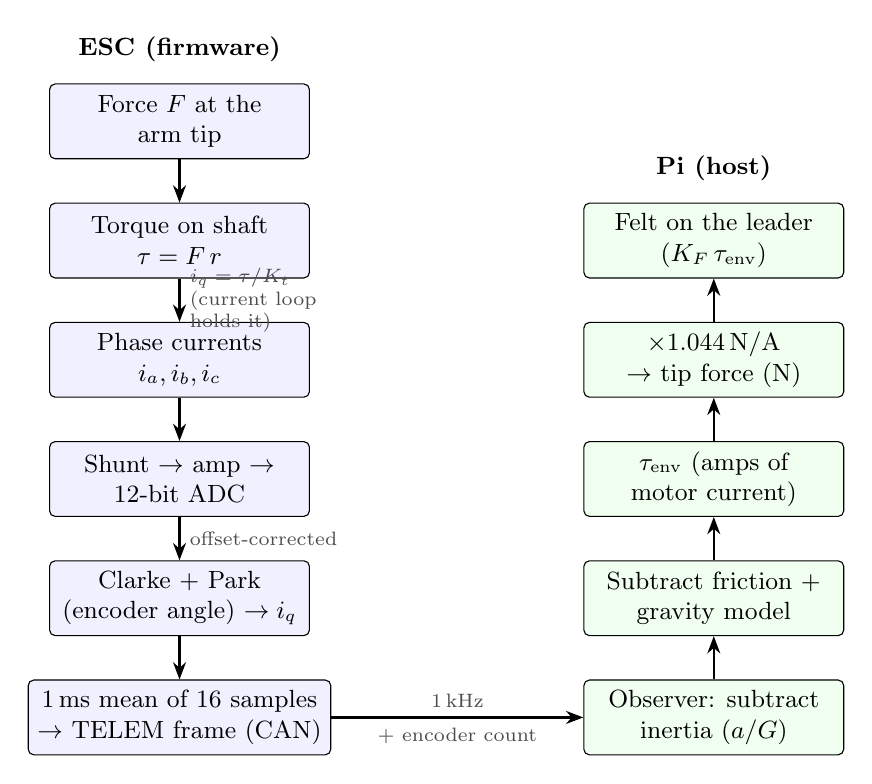
\begin{tikzpicture}[
  box/.style={draw, rounded corners=2pt, align=center, minimum width=3.3cm,
              minimum height=0.95cm, font=\small, fill=#1},
  box/.default={white},
  arr/.style={-{Stealth[length=2.2mm]}, thick},
  lab/.style={font=\scriptsize, align=left, text=black!70},
  node distance=0.55cm and 0.9cm]
  % ESC column
  \node[box=blue!6] (f)   {Force $F$ at the\\arm tip};
  \node[box=blue!6, below=of f] (tau) {Torque on shaft\\$\tau = F\,r$};
  \node[box=blue!6, below=of tau] (ph) {Phase currents\\$i_a,i_b,i_c$};
  \node[box=blue!6, below=of ph] (adc) {Shunt $\to$ amp $\to$\\12-bit ADC};
  \node[box=blue!6, below=of adc] (park) {Clarke + Park\\(encoder angle) $\to \iq$};
  \node[box=blue!6, below=of park] (mean) {1\,ms mean of 16 samples\\$\to$ TELEM frame (CAN)};
  % Pi column
  \node[box=green!6, right=3.2cm of mean] (obs) {Observer: subtract\\inertia ($a/G$)};
  \node[box=green!6, above=of obs] (fric) {Subtract friction +\\gravity model};
  \node[box=green!6, above=of fric] (tenv) {$\tau_{\mathrm{env}}$ (amps of\\motor current)};
  \node[box=green!6, above=of tenv] (newt) {$\times 1.044\NpA$\\$\to$ tip force (N)};
  \node[box=green!6, above=of newt] (felt) {Felt on the leader\\($K_F\,\tau_{\mathrm{env}}$)};

  \draw[arr] (f) -- (tau);
  \draw[arr] (tau) -- node[lab, right] {$\iq=\tau/K_t$\\(current loop\\holds it)} (ph);
  \draw[arr] (ph) -- (adc);
  \draw[arr] (adc) -- node[lab, right] {offset-corrected} (park);
  \draw[arr] (park) -- (mean);
  \draw[arr] (mean) -- node[lab, above] {1\,kHz} node[lab, below] {+ encoder count} (obs);
  \draw[arr] (obs) -- (fric);
  \draw[arr] (fric) -- (tenv);
  \draw[arr] (tenv) -- (newt);
  \draw[arr] (newt) -- (felt);

  \node[font=\small\bfseries, above=0.15cm of f] {ESC (firmware)};
  \node[font=\small\bfseries, above=0.15cm of felt] {Pi (host)};
\end{tikzpicture}
\caption{The force-sensing chain. Every arrow is a place where error can
enter; the sections below follow it from top-left to top-right.}
\label{fig:chain}
\end{figure}

%=====================================================================
\section{Physics: torque, current and force}
%=====================================================================

\subsection{Why only $\iq$ makes torque}

Field-oriented control (FOC) describes the three phase currents as one
current vector expressed in a frame that rotates with the rotor magnets.
Its two components are
\begin{itemize}
  \item $i_d$, aligned with the magnet flux. It makes no torque; the
        firmware holds it at zero.
  \item $\iq$, at $90^\circ$ electrical to the flux. All the torque comes
        from it:
        \begin{equation}
          \tau_{\mathrm{motor}} = K_t\,\iq .
          \label{eq:kt}
        \end{equation}
\end{itemize}
$K_t$ is the torque constant. The nominal value used in the plan brief is
$66\,\mathrm{mN\,m/A}$; the B7 static calibration measured
$64.6\,\mathrm{mN\,m/A}$ \measured.

\subsection{From torque to force at the tip}

A force $F$ pressing perpendicular to the arm at radius $r$ makes a torque
$\tau = F r$. If the arm is still, the motor must supply the opposite
torque, so
\begin{equation}
  F = \frac{K_t}{r}\,|\iq| .
  \label{eq:force}
\end{equation}
The ratio $K_t/r$ is the \emph{force factor} in N per amp. It depends on
\emph{where} the arm is pressed: the same 0.5\,A means 0.20\,N at
$r = 160\,\mathrm{mm}$ and 0.53\,N at $r = 75.7\,\mathrm{mm}$. This is why
the test log suggests stating thresholds as torque, which does not depend
on the contact point.

\subsection{When the arm moves: Newton's second law}

With the arm free to move, the current also has to accelerate the arm's
inertia $J$, fight friction, and hold up gravity:
\begin{equation}
  J\,\ddot\theta \;=\; K_t\,\iq \;-\; \tau_{\mathrm{fric}}(\dot\theta)
  \;-\; \tau_{\mathrm{grav}}(\theta) \;-\; \tau_{\mathrm{ripple}}(\theta,\iq)
  \;+\; \tau_{\mathrm{ext}} .
  \label{eq:newton}
\end{equation}
Solving for the external torque:
\begin{equation}
  \tau_{\mathrm{ext}} \;=\; J\,\ddot\theta \;-\; K_t\,\iq
  \;+\; \tau_{\mathrm{fric}} + \tau_{\mathrm{grav}} + \tau_{\mathrm{ripple}} .
  \label{eq:text}
\end{equation}
Everything on the right is either measured ($\iq$, $\theta$ from the
encoder) or modelled (friction, gravity, ripple, $J$). Section~\ref{sec:observer}
shows how the host evaluates this without differentiating noise twice.

\paragraph{Working in amps.} The host never converts to N\,m internally.
Dividing \eqref{eq:text} by $K_t$ gives everything in ``amps of equivalent
motor current''. The inertia becomes the \emph{plant gain}
\[
  G = \frac{K_t}{J}\cdot\frac{4000}{2\pi}
  \quad\text{(encoder counts/s}^2\text{ per amp)},
\]
which is measured directly instead of computing $J$. For the 3D-printed
follower arm $G = 3.85\times10^{6}$ counts/s$^2$ per A \measured. That
implies $J \approx 1.1\times10^{-5}\,\mathrm{kg\,m^2}$ \inferred.

%=====================================================================
\section{Measuring phase current on the ESC}
%=====================================================================

\subsection{Shunts, amplifier, ADC}

The B-G431B-ESC1 has a 3\,m$\Omega$ shunt resistor in the low-side leg of
each of the three phases. When a low-side transistor conducts, that
phase's current flows through its shunt and makes a small voltage. The
STM32's internal op-amp (programmable gain amplifier, PGA) amplifies it,
the board's input network adds a bias so negative currents can be read,
and the 12-bit ADC converts it.

\begin{table}[h]
\centering
\begin{tabular}{@{}lll@{}}
\toprule
Quantity & Value & Where \\
\midrule
Shunt $R_{\mathrm{shunt}}$ & $3\,\mathrm{m\Omega}$ & \file{power\_stage\_parameters.h} \\
PGA gain & $16\times$ (was $8\times$) & \file{main.c} OPAMP config \\
Net gain incl.\ input network & $16 \times 0.571 = 9.14$ & \file{AMPLIFICATION\_GAIN} \\
Volts at the ADC per amp & $0.003 \times 9.14 = 27.4\,\mathrm{mV/A}$ & \\
Zero-current level & $\approx 2.06\,\mathrm{V}$ & dev review 2026-10-28 \\
ADC full scale & $3.3\,\mathrm{V}$, 12 bits & \\
One ADC step & $3.3/4096/0.0274 = 29.4\mA$ & \\
Readable range (firmware) & $\pm 60.2\A$ & \file{M1\_MAX\_READABLE\_CURRENT} \\
Motor rating & $0.8\A$ & \file{NOMINAL\_CURRENT\_A} \\
\bottomrule
\end{tabular}
\caption{The current-sense front end, after the 16$\times$ gain change.}
\label{tab:frontend}
\end{table}

\paragraph{Why the 16$\times$ gain change.} The board is built for motors
that draw tens of amps. This motor's whole working range, $\pm0.8\A$, is
about 1\,\% of the readable range. At 8$\times$ one ADC step was
$58.8\mA$, so a 0.8\,A signal used only about 14 steps. Doubling the gain
halves the step to $29.4\mA$. It does not change the force; it improves
the resolution of the reading. (It also changed the meaning of the
over-current trip threshold; see CHANGE 6 in
\file{FIRMWARE\_CHANGES.txt}.)

\paragraph{Keep the gain in sync.} The gain appears in three places that
the compiler does not tie together: the OPAMP setting in \file{main.c},
\file{AMPLIFICATION\_GAIN}, and the current-PI gains in
\file{drive\_parameters.h}. The \file{.ioc}/\file{.stwb6} files still say
8$\times$, so regenerating the project from Motor Control Workbench would
silently revert all of it.

\subsection{Offsets: what ``zero amps'' reads as}
\label{sec:offset}

At zero current each channel reads its bias level, near 2.06\,V, but not
exactly the same level on every channel. The firmware subtracts a
per-channel \emph{offset} measured at START. A small offset error
$\delta$ on one phase looks like a constant current of $\delta$ in the
stationary frame. After the Park transform (Section~\ref{sec:park}) a
constant vector becomes a sine at the electrical frequency:
\begin{equation}
  \Delta\iq(\theta_e) = -\delta_\alpha \sin\theta_e + \delta_\beta\cos\theta_e
  = |\delta|\cos(\theta_e + \varphi).
\end{equation}
With 7 pole pairs, that is a torque ripple at \textbf{7 per mechanical
revolution}. You feel it as detents every $51^\circ$ on the leader.

What has been done about it:
\begin{itemize}
  \item \textbf{CHANGE 3:} average 128 samples instead of 16 for the offset
        (\file{NB\_CONVERSIONS}). This cuts the random part about
        $2.8\times$. It did not fix the 7/rev, which turned out to be
        systematic \measured.
  \item \textbf{CHANGE 5:} calibrate with the bridge switching at 50\,\%
        duty (zero net current), so the offsets are measured in the same
        conditions as RUN, and calibrate phase C separately on each of its
        two ADC paths (ADC1 ch12 and ADC2 ch18; they differed by 62--76
        counts $\approx 114$--$140\mA$) \measured.
  \item What remains: the 7/rev still grows during RUN (about 11 to
        $55\mA$ over 89\,s as the board warms from 34 to $40^\circ$C). The
        likely cause is offset drift with board temperature after
        calibration \inferred. A temperature-compensated offset is a
        candidate future change.
\end{itemize}

\paragraph{Gotcha: idle Iq is garbage.} Until a board has been STARTed
once after power-up there are no offsets, and TELEM reads about
$\pm25\A$ at rest. Never trust $\iq$ from a board that has not been
STARTed since power-up.

\subsection{When to sample: the PWM window}
\label{sec:sampling}

A low-side shunt only carries current while its low-side transistor is
on. The inverter switches at 16\,kHz with center-aligned PWM. Around the
middle of each period all three low sides are on, and that is when the
ADC samples (Figure~\ref{fig:pwm}).

\begin{figure}[h]
\centering
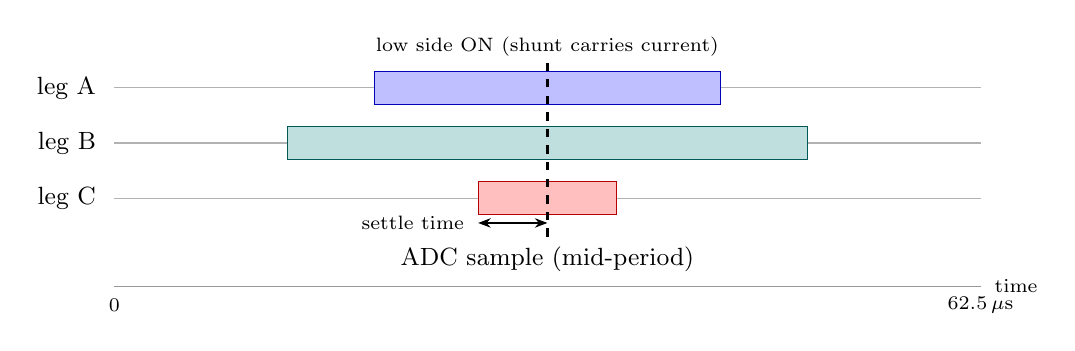
\begin{tikzpicture}[x=1.1cm, y=0.7cm, font=\small]
  % phases: low-side ON window centered at 5
  \foreach \name/\y/\w/\col in {A/3/4.0/blue, B/2/6.0/teal, C/1/1.6/red} {
    \node[anchor=east] at (-0.1,\y) {leg \name};
    \draw[black!30] (0,\y) -- (10,\y);
    \fill[\col!25] ({5-\w/2},\y-0.3) rectangle ({5+\w/2},\y+0.3);
    \draw[\col!70!black] ({5-\w/2},\y-0.3) rectangle ({5+\w/2},\y+0.3);
  }
  \node[font=\scriptsize, align=center] at (5,3.75) {low side ON (shunt carries current)};
  % sample point
  \draw[dashed, thick] (5,0.3) -- (5,3.45);
  \node[below] at (5,0.3) {ADC sample (mid-period)};
  % settle time from C edge
  \draw[{Stealth[length=1.6mm]}-{Stealth[length=1.6mm]}] (4.2,0.55) -- (5,0.55);
  \node[font=\scriptsize, anchor=east] at (4.15,0.55) {settle time};
  \draw[black!40] (0,-0.6) -- (10,-0.6);
  \node[font=\scriptsize, anchor=west] at (10.05,-0.6) {time};
  \node[font=\scriptsize] at (0,-0.95) {0};
  \node[font=\scriptsize] at (10,-0.95) {$62.5\,\mu$s};
\end{tikzpicture}
\caption{Schematic of one PWM period. Higher duty on a leg means a shorter
low-side window. Here leg C has the highest duty: its low side turns on
just before the sample, and its switching edge disturbs the other
channels. The time from that edge to the sample must exceed the
front-end's settling time.}
\label{fig:pwm}
\end{figure}

Because $i_a + i_b + i_c = 0$, the firmware needs only two phases and
computes the third. MCSDK's three-shunt driver has two strategies:
\begin{description}
  \item[Forced sector 5.] Read A and B at mid-period. Used while the
        window is wide enough, i.e.\ while the gap from the highest-duty
        leg's edge to mid-period is larger than a threshold
        \texttt{Tafter}.
  \item[Natural sector.] At higher duty, pick the two legs with the
        longest windows (the two lowest duties) and move the sample
        point accordingly.
\end{description}

\paragraph{What went wrong, and the fix.} Above about 0.55\,A at some
rotor angles, the measured $\iq$ read low and noisy, while the real
current (judged from the scale and from $V_q$) overshot: a 0.8\,A command
delivered about 0.93--0.96\,A \measured. The current PI loop regulates the
\emph{measured} current, so a reading that is low makes the loop push
harder. A measurement error is a force error. The sweep of \texttt{Tafter}
(CHANGE~7, SET\_PARAM over CAN) showed:
\begin{itemize}
  \item The error tracks the share of periods in \emph{natural-sector}
        mode. The forced A+B read is the accurate path, even with only
        $\approx 2.4\,\mu$s of settling \measured.
  \item Lowering \texttt{Tafter} from 807 counts ($4.75\,\mu$s) to 400
        ($2.35\,\mu$s) keeps the forced read up to 0.8\,A. Result: within
        2\,\% of command up to 0.8\,A at both a bad and a good angle, std
        26--$29\mA$ \measured.
  \item Why the natural-sector read is wrong is still open \inferred.
\end{itemize}
\texttt{Tafter} lives in RAM and resets to 807 on ESC reset, so the Pi
sends 400 before every START (\file{can\_interface.DEFAULT\_TAFTER}, env
\file{ESC\_TAFTER}).

\subsection{From three phase currents to $\iq$}
\label{sec:park}

Every 62.5\,$\mu$s the firmware:
\begin{enumerate}
  \item converts ADC counts to current: subtract the offset, scale by
        \file{CURRENT\_CONV\_FACTOR} (544 internal units per amp, so one
        internal unit is $1.84\mA$);
  \item Clarke transform: $i_\alpha = i_a$,\quad
        $i_\beta = (i_a + 2 i_b)/\sqrt3$;
  \item Park transform with the electrical angle $\theta_e$ from the
        encoder (4000 counts/rev, 7 pole pairs, so 571.4 counts per
        electrical revolution):
        \begin{equation}
          \iq = -i_\alpha\sin\theta_e + i_\beta\cos\theta_e .
        \end{equation}
\end{enumerate}
The encoder angle must be right for $\iq$ to mean ``torque current''.
That is why the first START after power-up runs a 2\,s, 0.8\,A alignment
(it locks the rotor to $90^\circ$ electrical, raw encoder 142). An angle
error $\epsilon$ would make the measured $\iq$ only $\cos\epsilon$ of the
real torque current.

\paragraph{Quantisation.} Because $\iq$ mixes two phase readings with
angle-dependent weights, its step is not a fixed $29.4\mA$. At one fixed
angle the values sat on a lattice with a step of about $16.5\mA$
\measured.

\subsection{Telemetry: the 1\,ms mean}

The current loop runs at 16\,kHz, but TELEM goes out at 1\,kHz. Originally
it carried one raw sample and dropped the other 15. With no anti-alias
filter, 0.5--8\,kHz noise folded into the 0--500\,Hz band. CHANGE~1 (plan
step B4) sends the mean of all 16 samples instead. A 16-tap boxcar has
nulls at exactly 1, 2, 3\,\ldots\,kHz, which are the frequencies that
alias to DC. Results \measured:
\begin{itemize}
  \item noise at 0\,A, follower free: $30.4\mA \to 3.1\mA$ std ($9.7\times$);
  \item step response unchanged (50\,\% at 1.45\,ms after the host send);
  \item averaging also dithers the lattice. The mean resolves much less
        than one ADC step.
\end{itemize}
The TELEM frame is \texttt{float32 Iq, uint16 encoder, uint16 \textmu s
clock}. The MCU timestamp is what the host uses for $dt$, so CAN jitter
does not corrupt velocity or acceleration.

%=====================================================================
\section{The host observer: separating contact from motion}
\label{sec:observer}
%=====================================================================

\subsection{The idea}

Rewrite \eqref{eq:text} in amps (divide by $K_t$, sign flipped so the
estimate is the external torque):
\begin{equation}
  \tau_{\mathrm{env}} \;=\; -\Bigl(\,\iq - \frac{a}{G} - m(\dot\theta,\theta)\Bigr),
\end{equation}
where $a$ is the shaft acceleration in counts/s$^2$ and $m$ is the
friction + gravity model. In words: \emph{the current that did not turn
into acceleration and was not used up by friction or gravity was pushing
against something.} At standstill $a = 0$, so $\tau_{\mathrm{env}} = -\iq$
(minus small model terms). The C2 test checked exactly that sign and
equality on 16 static holds \measured.

\subsection{Getting acceleration without double-differentiating noise}

Differentiating the encoder twice is very noisy. The observer (class
\file{ExternalTorqueObserver} in \file{estimators.py}) uses a low-pass filter
$L(s) = \omega/(s+\omega)$ with $\omega = 2\pi\cdot20\,\mathrm{Hz}$ and
the identity
\begin{equation}
  L(s)\,a \;=\; L(s)\,s\,v \;=\; \omega\bigl(v - L(s)\,v\bigr).
\end{equation}
So the filtered acceleration needs only velocity, not its derivative. The
observer computes
\begin{equation}
  \hat\tau_{\mathrm{motor}} \;=\; L\,\iq \;-\; \omega\bigl(x - L\,x\bigr),
  \qquad x = \frac{v}{G},
\end{equation}
which is $L(\iq - a/G)$: the same 20\,Hz filter on both terms, so they
stay consistent. A small factor
$1/(1-\pi f_c\,dt)$ corrects the discretisation, and $dt$ comes from the
MCU timestamps.

\subsection{The supporting pieces}

\begin{description}
  \item[Velocity] $v$: an $\alpha$--$\beta$ tracker on encoder counts
        (55\,Hz bandwidth) with a rest detector that outputs exactly 0
        when the encoder only dithers $\pm1$ count.
  \item[Time alignment] The velocity estimate lags about 2.6\,ms. If the
        current is not delayed to match, every acceleration shows up as a
        false force. The host delays $\iq$ by 3 frames (3\,ms). This cut
        the free-motion floor by 18\,\% \measured.
  \item[Plant gain] $G$ is fitted per arm from free-motion logs
        (\file{fit\_follower\_model.py}). Changing the arm changes $G$: the
        chopstick arm was $0.79\times10^6$, the 3D-printed arm
        $3.85\times10^6$. Using the wrong $G$ shows up as an error that
        grows with acceleration.
  \item[Friction + gravity model] $m(\dot\theta,\theta)$, fitted in
        \file{follower\_model\_arm3d.json}:
        offset $-1.7\mA$, Coulomb $24.5\mA$, low-speed correction
        $-26.9\mA$ (decays with $|v|$ over 1500 counts/s), viscous
        $2.3\mA$ per 10k counts/s, gravity $-13.5\cos\theta - 2.4\sin\theta$\,mA.
\end{description}

\subsection{How well it works}

\begin{table}[h]
\centering
\begin{tabular}{@{}lll@{}}
\toprule
Test & Result & Tip force (at $1.044\NpA$) \\
\midrule
Free-motion floor, vigorous swinging (C2 live) & $19.1\mA$ rms (p99 56) & $\approx 20\mN$ rms \\
Sensor noise alone (B4, at rest) & $3.1\mA$ std & $\approx 3\mN$ \\
Static accuracy vs measured current (C2) & worst 5.0\,\% & \\
Rigid contacts in teleop & 0.28--$0.85\A$ & 0.3--0.9\,N \\
\bottomrule
\end{tabular}
\caption{Observer performance on the 3D-printed follower arm.}
\end{table}

So contact stands out from free motion by roughly $15$--$45\times$ in RMS
terms.

\paragraph{The hard limit: stiction.} When the arm is stopped, static
friction can hold part of a load (breakaway is 0.05--0.09\,A on this rig,
about 100$\times$ what the original brief assumed). With no motion there
is no way to tell ``friction is holding it'' from ``something is pushing
on it''. The at-rest residual is about $18.7\mA$ and is the main reason
the brief's $15\mA$ target was not met \measured. In teleop, a 20\,mA dead
band on $\tau_{\mathrm{env}}$ keeps this from being felt.

%=====================================================================
\section{Calibrating to newtons}
%=====================================================================

The force factor in \eqref{eq:force} was measured by pressing the arm tip
on a kitchen scale with known commanded currents
(\file{b7\_force\_cal.py}):

\begin{table}[h]
\centering
\begin{tabular}{@{}llll@{}}
\toprule
Run & Arm / radius & Slope & Implied $K_t$ \\
\midrule
B7 (2026-10-25) & link, $r\approx160\,\mathrm{mm}$ & $0.404\NpA$ ($R^2$ 0.996) & $64.6\,\mathrm{mN\,m/A}$ \\
D1 static (2026-10-28) & 3D arm, $r = 75.7\,\mathrm{mm}$ & $1.044\NpA$ ($R^2$ 0.995) & $79\,\mathrm{mN\,m/A}$ \\
\bottomrule
\end{tabular}
\caption{Scale calibrations. Force reporting uses $1.044\NpA$
(\file{SHADOW\_N\_PER\_A} in \file{teleop\_test.py}).}
\end{table}

The two runs disagree by 22\,\% in $K_t$. Either B7's ``roughly 160\,mm''
radius was long, or the 3D arm's effective contact point is closer to the
shaft than 75.7\,mm \inferred. The 1.044\,N/A figure was measured on the
arm actually in use, so it is the one used. It was fitted on levels up to
0.45\,A, before the \texttt{Tafter} fix. The scale check up to 0.8\,A with
\texttt{Tafter} 400 is still to do.

\paragraph{The motor mount must be rigid.} In the 4\,cm rerun the mount
visibly moved under load. A compliant mount absorbs part of a push and
makes a rigid contact look soft, which corrupts both the force factor and
any stiffness measurement.

\paragraph{The feel does not depend on this number.} In teleop the felt
force is current-to-current (follower amps $\to$ leader amps), so the N/A
factor only affects the numbers in the logs and plots, not what you feel.

%=====================================================================
\section{Teleoperation: how force is passed between the motors}
\label{sec:teleop}
%=====================================================================

The teleoperation loop runs on the Pi at 500\,Hz in
\file{ESC\_based/software/teleop\_test.py}. Motor~A (ESC~1) is the
\emph{follower}; its arm touches the object. Motor~B (ESC~2) is the
\emph{leader}; the operator turns it. Every tick the Pi sends each ESC one
current command (\texttt{SET\_IQ}), and every quantity below is in amps of
motor current. Each addition is behind a \texttt{TELEOP\_*} environment
variable whose default is off, so with no flags the script behaves like
the original in \file{software/}.

\subsection{Where it started: the ``echo'' finding}
\label{sec:echo}

\begin{figure}[h]
\centering
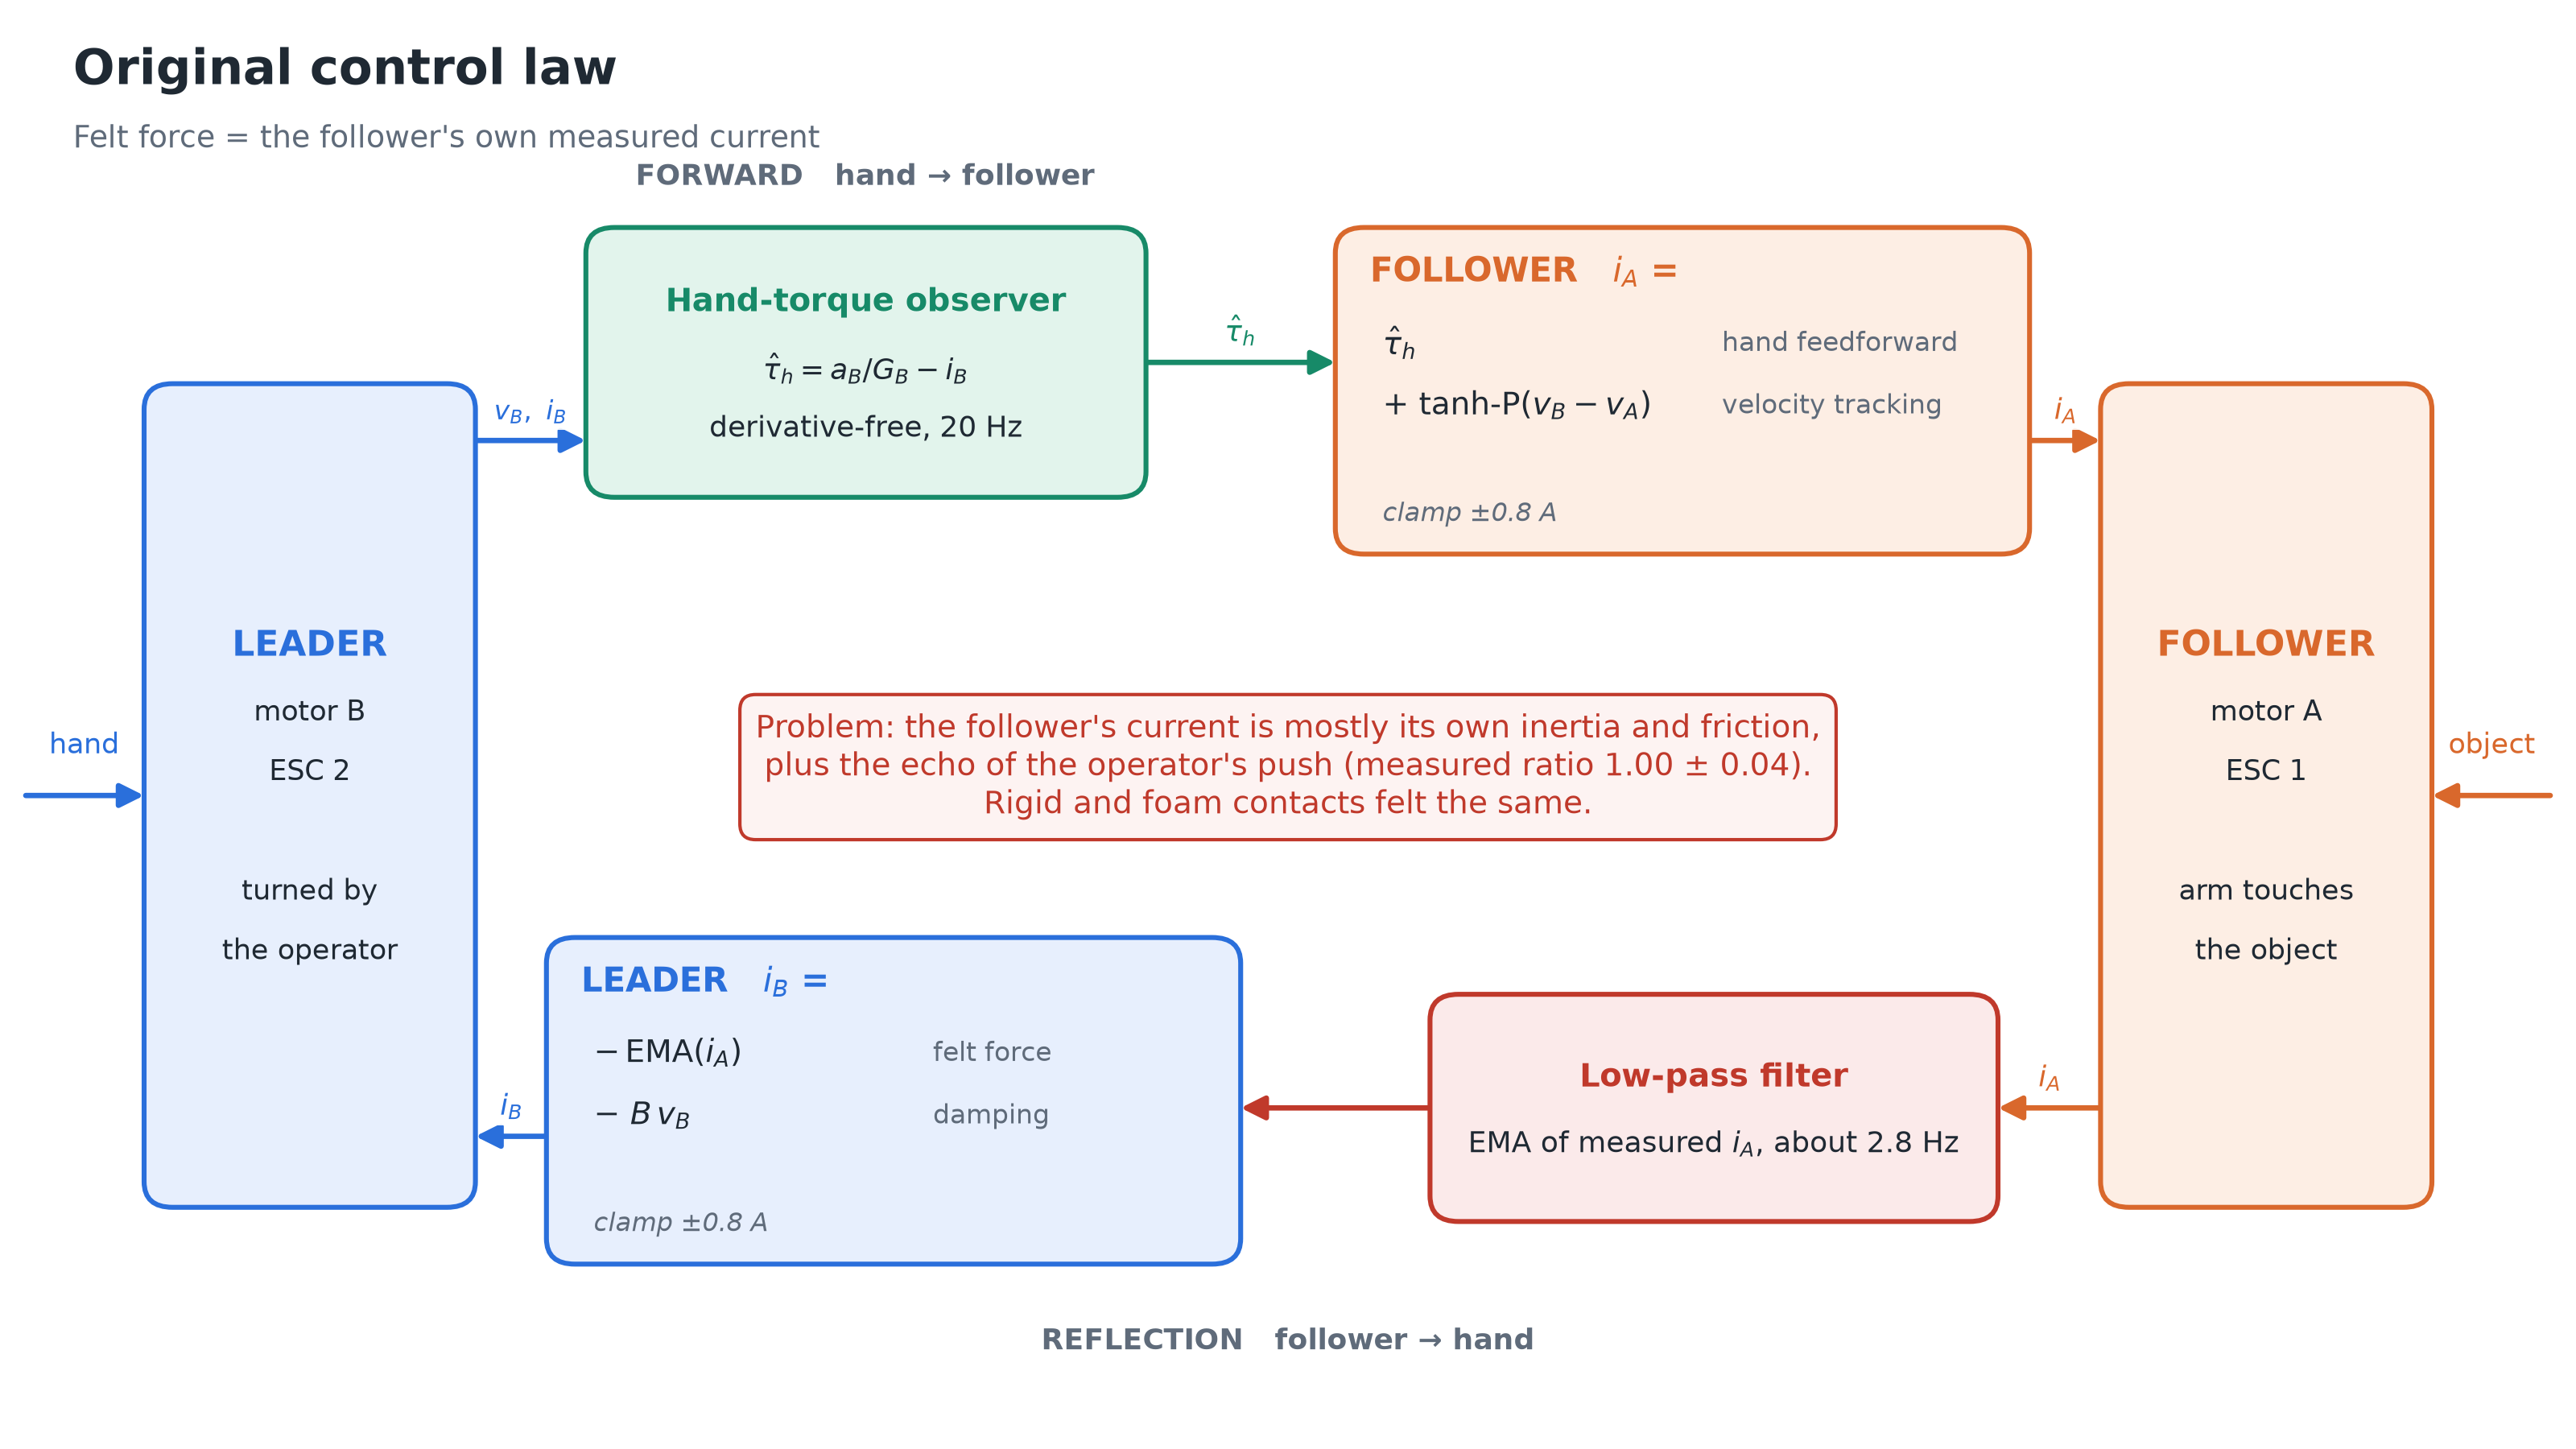
\includegraphics[width=\linewidth]{diagram_original.png}
\caption{The original control law. The forward path already had the
hand-torque observer; the reflection path sent the follower's low-pass
filtered \emph{raw current} to the leader.}
\label{fig:original}
\end{figure}

In the original law (Figure~\ref{fig:original}) the leader was commanded
$i_B = -\mathrm{EMA}(i_{q,A}) - K_B v_B$, with a 2.8\,Hz filter. In every
hand-clamp and foam press, the felt current equalled minus the operator's
own hand torque (ratio $1.00\pm0.04$; a fit over 18k ticks of each of the
table and foam runs gives slope $-1.01$, $r=-0.997$), and 95--125\,\% of
the follower's command was feedforward copying the operator's motion. The
operator felt their own push echoed back, and a table and a block of foam
felt the same \measured. Free-space RMS felt current was $116\mA$ and the
contact rise time (10--90\,\%) was 66\,ms. Subtracting the part of the
current that only accelerates the arm ($a/G$) and the friction model is
what turns ``current'' into ``environment force''
(Section~\ref{sec:observer}).

\subsection{The current control law}

\begin{figure}[h]
\centering
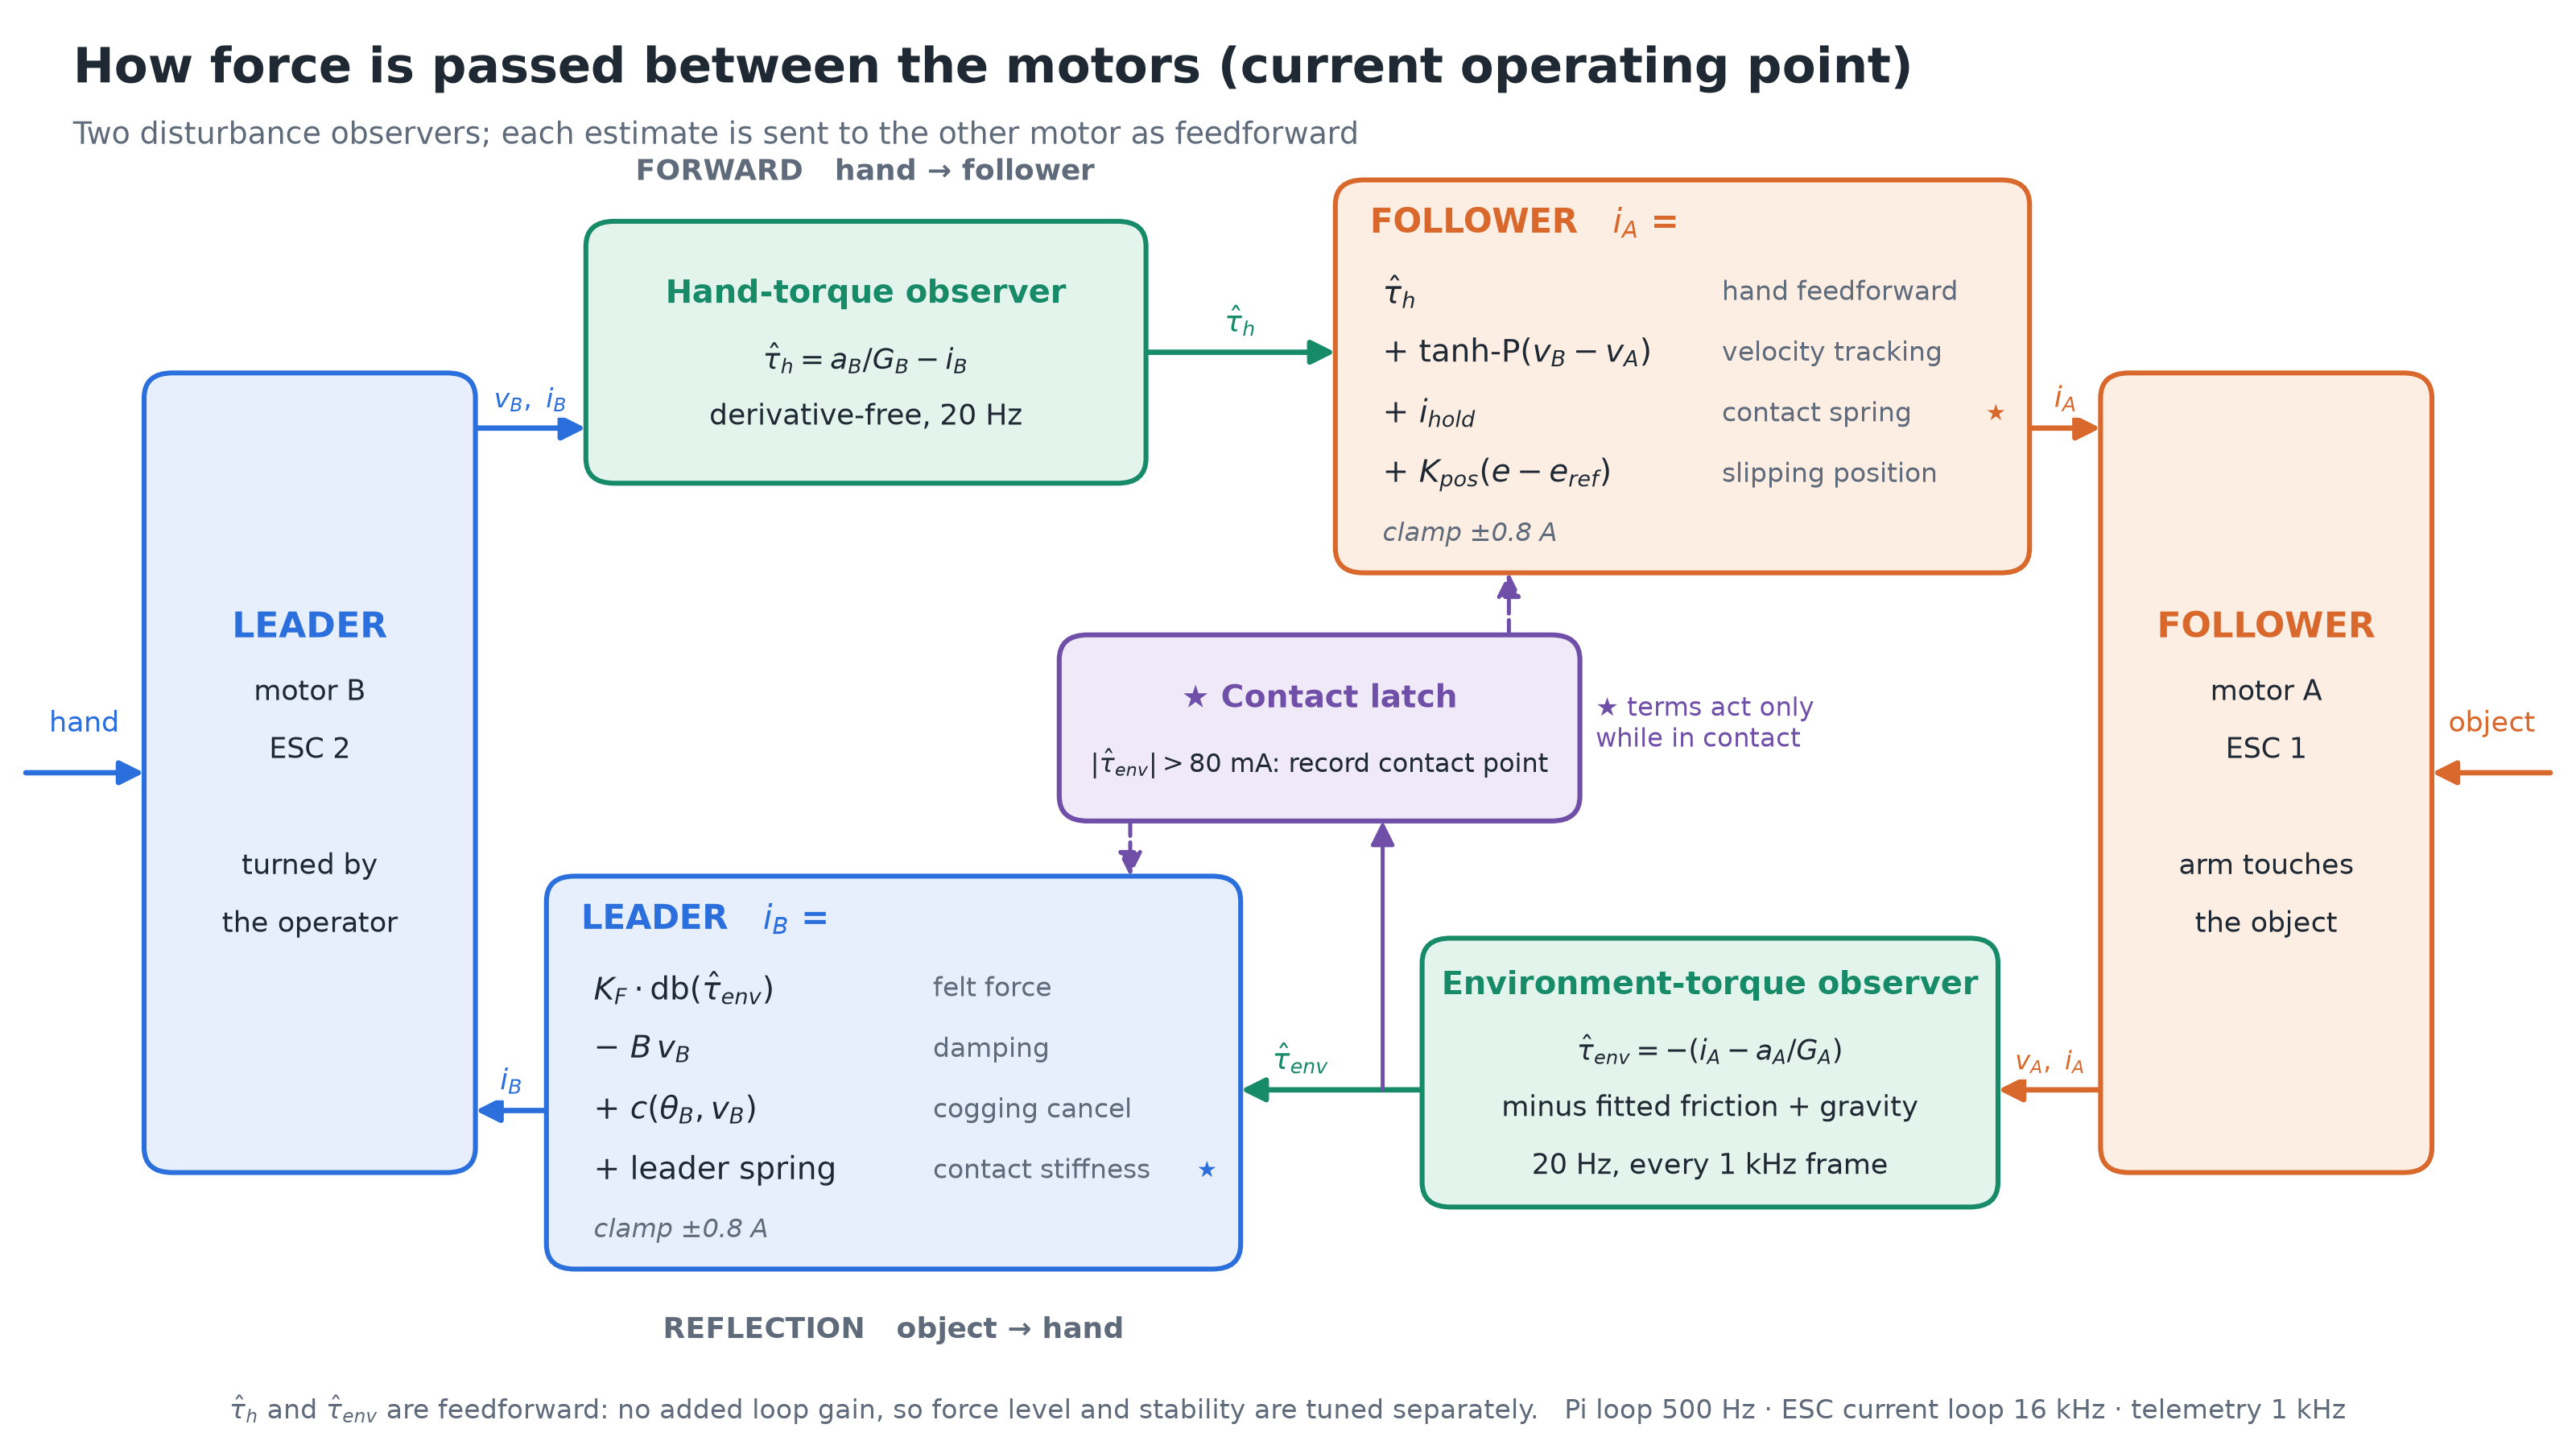
\includegraphics[width=\linewidth]{diagram_control.png}
\caption{The current operating point. Two disturbance observers; each
estimate is sent to the other motor as feedforward. Starred terms act only
while a contact is latched.}
\label{fig:control}
\end{figure}

With $e = \Delta\theta_B - \Delta\theta_A$ the leader-minus-follower
displacement (counts since the start of the run) and $\sigma = +1$ the
sign convention on this rig, the two commands are
\begin{align}
  i_A &= \mathrm{clamp}_{0.8\A}\Bigl(
        \underbrace{I_{\max}\tanh\!\Bigl(\tfrac{K_v (v_B - v_A)}{I_{\max}}\Bigr)}_{\text{velocity tracking}}
        + \underbrace{\hat\tau_h}_{\text{hand feedforward}}
        + \underbrace{i_{\mathrm{hold}}}_{\text{contact spring}^\star}
        + \underbrace{i_{\mathrm{pos}}}_{\text{slipping position}}\Bigr),
  \label{eq:iA}\\
  i_B &= \mathrm{clamp}_{0.8\A}\Bigl(
        \underbrace{K_F\,\mathrm{DB}_\delta(\tau_{\mathrm{env}})}_{\text{felt force}}
        - \underbrace{K_B\,v_B}_{\text{damping}}
        + \underbrace{d_L(\theta_B, v_B)}_{\text{cogging + friction}}
        + \underbrace{i_{L}}_{\text{leader spring}^\star}\Bigr).
  \label{eq:iB}
\end{align}
The subsections below take the terms one at a time.

\begin{table}[h]
\centering
\small
\begin{tabular}{@{}>{\raggedright}p{3.4cm}>{\raggedright}p{4.6cm}>{\raggedright}p{2.3cm}>{\raggedright\arraybackslash}p{3.3cm}@{}}
\toprule
Term & Purpose & When active & Added \\
\midrule
$\hat\tau_h$ (follower) & reproduce the hand's push on the follower & always & original \\
velocity tracking (follower) & keep the follower moving with the leader & always & original \\
$K_F\,\mathrm{DB}(\tau_{\mathrm{env}})$ (leader) & felt force = environment estimate & always & C3, 2026-10-25 \\
$K_B v_B$ (leader) & damping of the reflection loop & always & original (retuned in C3) \\
$d_L$ (leader) & cancel the leader's cogging and friction & always & 2026-10-26 \\
$i_{\mathrm{hold}}$ (follower) & stop held presses fading & in contact & 2026-10-26 \\
$i_L$ (leader) & stop the leader at the contact & in contact & 2026-10-29 \\
$i_{\mathrm{pos}}$ (follower) & stop the follower drifting & always & 2026-10-29 \\
\bottomrule
\end{tabular}
\caption{The terms of \eqref{eq:iA} and \eqref{eq:iB}.}
\end{table}

\subsection{Forward path: the hand-torque observer on the leader}

The leader obeys the same plant as the follower,
$\dot v_B = G_B\,(i_B + \tau_h + \tau_{d,B})$, where $\tau_h$ is the hand
torque and $\tau_{d,B} = -d_L$ the leader's own cogging and friction, all
in amps. The observer has the same derivative-free form as the follower's
(Section~\ref{sec:observer}), with $x_B = v_B/G_B$ and the same 20\,Hz
filter $L$:
\begin{equation}
  \hat\tau_h = \omega\bigl(x_B - L\,x_B\bigr) - L\bigl(i_{q,B} - d_L\bigr)
  \;=\; L\Bigl(\frac{a_B}{G_B} - i_{q,B} + d_L\Bigr).
\end{equation}
It uses the leader's \emph{measured} current and $G_B = 7.915\times10^6$
counts/s$^2$ per A. (The A2 re-identification measured
$9.672\times10^6$, 22\,\% higher; the user chose not to apply it yet.)
The follower receives $\hat\tau_h$ directly (gain 1, clamped to
$\pm1\A$), so the follower pushes on the object with the torque the hand
puts on the leader.

\paragraph{Why it is feedforward, and why it is not positive feedback.}
A velocity loop alone can only make force from a velocity error, and a
static push has none. Earlier tuning showed that a stiff velocity loop
delivered force only by running past its stability limit, in a
25--35\,Hz limit cycle \measured. $\hat\tau_h$ adds no loop gain, so force
level and stability become separate settings, and it works at zero
velocity. It looks like a loop, because $i_B$ appears in it, but when
$i_B$ changes the leader accelerates and the $a_B/G_B$ term cancels the
change. The residual loop gain is roughly the fractional error in $G_B$
\inferred.

\subsection{Velocity tracking on the follower}

\[
  i_{\mathrm{vel}} = I_{\max}\tanh\!\Bigl(\frac{K_v\,(v_B - v_A)}{I_{\max}}\Bigr),
  \qquad K_v = 3\times10^{-5}\ \mathrm{A/(count/s)},\quad I_{\max}=0.8\A .
\]
The $\tanh$ keeps the small-signal slope $K_v$ but bends smoothly toward
the ceiling instead of hard-clipping. The derivative term is zeroed.
This term only keeps the follower moving with the leader in free space;
it holds no position, which is why the follower drifted until the slipping
position coupling was added (Section~\ref{sec:poscoupling}).

\subsection{Reflection path: the felt force}

\begin{equation}
  i_{B,\mathrm{felt}} = K_F\,\mathrm{DB}_\delta(\tau_{\mathrm{env}}) - K_B\,v_B,
  \qquad \mathrm{DB}_\delta(x) = \operatorname{sign}(x)\max(0,|x|-\delta),
\end{equation}
with $K_F = 1.0$, $\delta = 20\mA$ and $K_B = 0.35\times10^{-5}$
A/(count/s). In a static press $\tau_{\mathrm{env}} = -i_{q,A}$, so at
$K_F=1$ the leader pushes back with the same current, and so the same
torque, as the follower (the motors are identical). In free space
$\tau_{\mathrm{env}}\approx 0$, so the operator feels almost nothing. The
dead band hides the follower's stiction at rest. $K_B = 0.25\times10^{-5}$
oscillated in contact; $0.5\times10^{-5}$ is the conservative fallback.
Results (C3) \measured: free felt current $18.7\mA$ RMS (from $116\mA$),
tap rise median 4\,ms (from 66\,ms).

\subsection{Leader calibration: ripple and friction in one fit}
\label{sec:leadercal}

Turned by hand, the leader is not smooth: cogging and torque ripple make
it snap at certain angles, and it has friction. Uncompensated, the operator
feels the bumps, and the hand observer mistakes them for hand torque and
forwards them to the follower.

\paragraph{Why every session.} Two parts of the ripple change: the 7/rev
part (once per electrical cycle, an offset error,
Section~\ref{sec:offset}) changes size on every START, and the 12/rev part
is locked to the stator, so its phase in encoder counts depends on which
of the 7 electrical zeros the power-up alignment landed on \measured. A
fixed map cannot follow either, so a fit is made right after START
(\file{leader\_cal.py}, \texttt{TELEOP\_LEADER\_CAL=1}).

\paragraph{The sweep.} Hands off, follower at 0\,A. The leader is held in
a position loop ($K_p = 10^{-3}$\,A/count, $K_d = 1.2\times10^{-5}$,
at most 0.3\,A) whose target moves one revolution forward at a constant
$300$ counts/s, pauses, and comes back (about 30\,s). Every 1\,kHz frame
records angle, measured current and reference speed. It aborts, and
teleop does not start, on a lag over 300 counts, a speed over 8000
counts/s, or stale telemetry.

\paragraph{The physics.} With no hand on the leader and constant speed,
$\dot v = 0$ in the plant, so
\begin{equation}
  0 = G_B\bigl(\iq + \tau_{d}\bigr) \;\Longrightarrow\; \iq = -\tau_d \equiv d(\theta, v):
\end{equation}
the current the position loop supplies \emph{is} the disturbance. Only
constant-speed frames are used; the ramps would add inertia current.

\paragraph{Separating ripple from friction.} Ripple depends on angle and
not on direction; friction depends on direction and not on angle. With
$r(\theta)$ the ripple and $f$ the Coulomb friction,
\begin{align}
  \text{forward:}\quad  i_{+}(\theta) &= c_0 + f + r(\theta), \\
  \text{backward:}\quad i_{-}(\theta) &= c_0 - f + r(\theta),
\end{align}
so $\tfrac12(i_+ + i_-) = c_0 + r(\theta)$ and $\tfrac12(i_+ - i_-) = f$.
Sweeping both directions over the same angles is what separates them.

\paragraph{The fit.} Rather than a lookup table, the ripple is a short
Fourier series at the harmonics found in Phase A, and everything is fitted
at once by linear least squares over the constant-speed frames
($\approx 20$k):
\begin{equation}
  \iq = c_0 + f\,\operatorname{sign}(v) + \sum_{h\in H}
        \bigl[a_h\cos(h\theta) + b_h\sin(h\theta)\bigr],
  \qquad H = \{7,12,14,24,28,36,42,84\},
\end{equation}
with $\theta = 2\pi\,(\text{count} \bmod 4000)/4000$. That is 18 unknowns,
$\mathbf c = \arg\min\|X\mathbf c - \mathbf i\|^2$. Each raw sample carries
30--43\,mA of noise, about the size of the ripple itself; a table with one
bin per angle would record mostly noise. Restricting the fit to known
harmonics averages the noise out and interpolates between samples.

\paragraph{How it is used.} The compensation term is
\begin{equation}
  d_L(\theta, v) = g_r\sum_{h\in H}\bigl[a_h\cos h\theta + b_h\sin h\theta\bigr]
                 + g_f\,f\tanh(v/v_0),
\end{equation}
with $g_r = 1$, $g_f = 0.5$ and $v_0 = 300$ counts/s. $c_0$ is dropped (it only absorbs a constant bias). $\tanh$ replaces
$\operatorname{sign}$ so the friction term does not flip abruptly at
standstill. Friction is compensated at half strength so the feedforward
(about 8\,mA) stays below the real friction (17\,mA running, 13--50\,mA
breakaway) and cannot start the leader on its own \inferred. $d_L$ is used
twice: added to the leader command (the motor supplies its own cogging, so
the operator does not feel it), and subtracted from $i_{q,B}$ inside the
hand observer (so the bumps are not forwarded to the follower).

\paragraph{Results} (LCAL1, 2026-10-26) \measured: fitted 12/rev
$35.8\mA$, 28/rev $13.1\mA$, 36/rev $8.1\mA$, Coulomb $16.2\mA$;
angle-locked RMS $28.8 \to 11.0\mA$ after the fit; the 12/rev leader speed
ripple felt in teleop fell from about 50\,\% to about 15\,\% of speed. The
user reported that it ``felt better''. \emph{Limit:} the 7/rev part grows for
minutes after START (time constant $\approx 160$\,s, to about 60\,mA warm;
thermal offset drift \inferred), so a START-time fit underestimates it.
\texttt{TELEOP\_LEADER\_WARMUP\_S} can hold both motors at 0\,A first; it
is off by default.

\subsection{Follower contact spring: holding a press}
\label{sec:holdspring}

\paragraph{The problem.} In a static press the force goes round a loop:
hand $\to\hat\tau_h\to$ follower pushes the object $\to\tau_{\mathrm{env}}\to$
leader pushes the hand $\to\hat\tau_h$. Its gain is $K_F\cdot 1 = 1$, and
nothing ties the force level to how far the leader is pushed in. Each pass
loses a fixed amount to the dead band and to friction, so a held press
decayed nearly linearly to zero in 1--1.5\,s, at 0.4--0.56\,A/s
\measured.

\paragraph{The law} (\file{contact\_spring.py}). At contact onset,
$|\tau_{\mathrm{env}}| > 0.08\A$, latch $e_0 = e$, the push direction
$s = -\operatorname{sign}(\tau_{\mathrm{env}})$ and the time $t_0$. While
latched,
\begin{equation}
  i_{\mathrm{hold}} = s\,\rho(t)\,\mathrm{clamp}_{[0,\,i_{\max}]}\bigl(s\,k\,(e - e_0)\bigr),
  \qquad \rho(t) = \min\!\Bigl(1, \frac{t - t_0}{T_r}\Bigr),
\end{equation}
with $k = 0.5\times10^{-3}$\,A/count, $i_{\max} = 0.05\A$ and
$T_r = 0.3$\,s. The spring pushes only toward the object, and only once
the leader is past the point where contact began. It releases when
$|\tau_{\mathrm{env}}|$ stays below 0.04\,A for 50\,ms, or when the
follower moves faster than 3000 counts/s (a false engage or a bounce).

\paragraph{Why a small spring is enough.} The circulating loop integrates
any excess over the leak, so $i_{\mathrm{hold}}$ does not set the held
force. The force settles where the spring just refills the leak,
$e - e_0 \approx \text{leak}/k$, a few tens of counts. That pins the leader
at the contact point like a wall, and the hand sets the force level
\inferred. $i_{\max}$ bounds how fast force can wind up if the hand is held
rigidly past the contact point. The ramp $\rho$ is there because at full
strength from the first sample the spring doubled the leader's ringing in
the first 0.3\,s of contact \measured.

\paragraph{Result} \measured: hold slope $-0.3\ldots-0.5$\,A/s $\to$
$-0.03/{+0.02}$\,A/s; user: ``the holds feel solid''.

\subsection{Leader contact spring and damping: making rigid feel rigid}
\label{sec:leaderspring}

\paragraph{The problem} (D2 preview, 2026-10-29). The follower measured a
rigid object as $\geq 1.6$\,N/mm and a soft one as 0.17\,N/mm, $9.6\times$
apart (sponge: $19.9\times$). By feel, though, the operator could not tell
them apart. While the felt force built from 0.15 to 0.7\,N, the leader
travelled 382 counts ($34^\circ$) on the rigid object and 452--473 counts
on the soft ones, against 3 and 28--55 counts at the follower \measured.
The stiffness the operator felt was the coupling's own compliance (about
0.7\,N per $35^\circ$), not the object's.

\paragraph{The law.} On the same latch, the leader gets a one-way spring on
the same displacement, opposite in sign to the follower's push, plus
contact damping:
\begin{equation}
  i_L = -s\,\mathrm{clamp}_{[0,\,i_{L,\max}]}\bigl(s\,k_L\,(e - e_0)\bigr) - B_L\,v_B,
\end{equation}
with $k_L = 2\times10^{-3}$\,A/count, $i_{L,\max} = 0.4\A$ and
$B_L = 10^{-5}$\,A/(count/s), with no ramp. Because the follower is stopped
by the object, $e - e_0$ is how far the leader has gone past the contact
point.

\paragraph{Damping and passivity.} A virtual spring sampled every
$T = 2$\,ms can inject energy. The standard passivity condition for a
sampled virtual wall (Colgate and Schenkel) asks for
$B_L > k_L T/2 = 2\times10^{-6}$; $B_L = 10^{-5}$ gives a $5\times$ margin
(bus delay adds to the requirement \inferred) and costs only about 10\,mA at
1000 counts/s.

\paragraph{No wind-up.} The leader spring is not forwarded to the
follower: the hand observer measures the true hand torque, and the spring
current is supplied by the leader motor itself. An offline simulation
(\file{leader\_spring\_sim.py}) with a force-controlled hand held the force
at the hand's level with no creep to the cap. It predicted leader travel
427 $\to$ 41 counts at $k_L = 2\times10^{-3}$ \inferred.

\paragraph{Results} (rigid object, median per press) \measured:
\begin{center}
\small
\begin{tabular}{@{}>{\raggedright}p{3.1cm}>{\raggedright}p{3.4cm}>{\raggedright}p{2.6cm}>{\raggedright\arraybackslash}p{5.2cm}@{}}
\toprule
Step & Leader travel, 0.15 $\to$ 0.7\,N & Leader velocity sign flips per press & User \\
\midrule
No leader spring & 382 counts ($34^\circ$) & 1 & ``couldn't tell'' \\
$k_L$ only & 50 counts ($4.5^\circ$) & 5 & ``best it has ever been'', minor ringing \\
$+\,B_L$ & 20 counts ($1.8^\circ$) & 3 (taps) & ``rang less'' \\
$+$ position coupling & 31 counts ($2.8^\circ$) & 5 & ``felt good'' \\
\bottomrule
\end{tabular}
\end{center}
The total leader command is still clamped at 0.8\,A, so above about
0.84\,N at the tip the leader gives way. The rigid-versus-soft feel test
has not been repeated with the leader spring yet.

\subsection{Slipping position coupling: stopping follower drift}
\label{sec:poscoupling}

\paragraph{The problem.} Velocity tracking matches speeds only, so with the
leader held still nothing holds the follower's position. The arm sagged
under gravity (model gravity $13.5\mA$, about the Coulomb level) in
10--20-count stick-slip steps, at 150--230 counts/s, and $e$ ratcheted to
thousands of counts over a run \measured.

\paragraph{The law.} A weak position spring whose reference slips:
\begin{equation}
  e_{\mathrm{ref}} \leftarrow \mathrm{clamp}_{[e - W,\; e + W]}\bigl(e_{\mathrm{ref}}\bigr),
  \qquad i_{\mathrm{pos}} = \sigma\,K_{\mathrm{pos}}\,(e - e_{\mathrm{ref}}),
\end{equation}
with $K_{\mathrm{pos}} = 10^{-3}$\,A/count and $W = 30$ counts, so
$|i_{\mathrm{pos}}| \le K_{\mathrm{pos}} W = 30\mA$ (about twice the gravity
term). Inside the window it is a spring that pulls the follower back into
line. Beyond the window the reference is dragged along, like a slipping
clutch, so the large leader-ahead gaps left after pushing through the
current cap are absorbed instead of yanking the follower.

\paragraph{Result} \measured: follower drift with the leader still, max
$167 \to 18$ counts/s (median $24\to 8$); free-motion felt current
unchanged ($36.3\to 38.4\mA$ on the same metric); in contact the term sits
at about $-20\mA$. User: ``it felt good \ldots\ there is still some drift,
but much improved''.

\subsection{The operating point}

\begin{table}[h]
\centering
\small
\begin{tabular}{@{}>{\raggedright}p{3.6cm}>{\raggedright}p{5.4cm}>{\raggedright\arraybackslash}p{6.2cm}@{}}
\toprule
Setting & Value & Environment variable \\
\midrule
Felt-force gain, dead band & $K_F = 1.0$, $\delta = 20\mA$ & \texttt{TELEOP\_K\_F}, \texttt{TELEOP\_FELT\_DEADBAND\_A} \\
Leader damping & $K_B = 0.35\times10^{-5}$ A/(count/s) & \texttt{TELEOP\_KB\_DAMP} \\
Follower contact spring & $k=0.5\times10^{-3}$, $i_{\max}=0.05\A$, $T_r = 0.3$\,s & \texttt{TELEOP\_HOLD\_K}, \texttt{\_MAX\_A}, \texttt{\_RAMP\_S} \\
Leader contact spring & $k_L = 2\times10^{-3}$, $0.4\A$, $B_L = 10^{-5}$ & \texttt{TELEOP\_LEADER\_K}, \texttt{\_K\_MAX\_A}, \texttt{\_CONTACT\_DAMP} \\
Slipping position coupling & $K_{\mathrm{pos}} = 10^{-3}$, $W = 30$ counts & \texttt{TELEOP\_POS\_K}, \texttt{TELEOP\_POS\_WINDOW} \\
Leader calibration & on, at each START & \texttt{TELEOP\_LEADER\_CAL=1} \\
Follower model & 3D-printed arm & \texttt{TELEOP\_FOLLOWER\_MODEL} \\
Current clamp & $\pm 0.8\A$ & \texttt{TELEOP\_IQ1\_MAX\_A} \\
ADC sampling delay & \texttt{Tafter} 400 & sent by \file{can\_interface} \\
\bottomrule
\end{tabular}
\caption{Operating point as of 2026-10-29. The full command is in
\file{TEST\_LOG.md}, ``0c UPDATE 3''.}
\end{table}

\subsection{Alternative architecture: coupling on the ESCs}

The ESC\_based firmware can also run the coupling on the ESCs themselves,
with the Pi out of the loop. Each ESC reads the other's TELEM frame off the
CAN bus and runs, every 1\,kHz tick,
\begin{equation}
  \iq = \mathrm{clamp}_{0.8\A}\Bigl(-\bigl[K_p\,(\Delta\theta_{\mathrm{own}} - \Delta\theta_{\mathrm{peer}})
       + K_d\,(v_{\mathrm{own}} - v_{\mathrm{peer}}) + K_{d,\mathrm{local}}\,v_{\mathrm{own}}\bigr]\Bigr),
\end{equation}
a classic position--position spring-damper with no force estimation. An
optional prediction couples to where the peer is now (last position plus
velocity $\times$ age). Runs on 2026-10-06 reached $K_p = 0.01$\,A/count,
about $38\times$ the 0.000265 of the Pi-side position mirror, with peer
data under 1\,ms old, but showed full-scale $\pm0.8\A$ buzzing at that
stiffness \measured. It has not been tuned or evaluated since. All the
force-feedback results in this document come from the Pi-side law above.

%=====================================================================
\section{Error budget and limits}
%=====================================================================

\begin{table}[h]
\centering
\small
\begin{tabular}{@{}>{\raggedright}p{3.6cm}>{\raggedright}p{3.4cm}>{\raggedright\arraybackslash}p{6.4cm}@{}}
\toprule
Source & Size & Status \\
\midrule
ADC quantisation & $29.4\mA$/step per phase & Dithered away by the 16-sample mean \\
Sensor noise (1\,ms mean) & $\approx 3\mA$ std at rest; 14--29\,mA under 0.3--0.8\,A stall & Fine for contact detection \\
Offset error (7/rev ripple) & 11 $\to$ $55\mA$ as the board warms & Partly fixed (CHANGES 3, 5); thermal drift open \\
Cogging/angle ripple (12, 24, 28, 36/rev) & up to $\approx 22\mA$ (12/rev) & Leader: in-session calibration cuts it 3--4$\times$ (Sec.~\ref{sec:leadercal}) \\
Sampling breakdown & up to $-15\,\%$ at 0.8\,A & Fixed with \texttt{Tafter} 400 (within 2\,\%) \\
Static friction & 0.05--0.09\,A breakaway & Fundamental: indistinguishable from load at rest \\
Inertia / timing mismatch & grows with $|a|$ & Fitted $G$ + 3\,ms current delay \\
Force factor uncertainty & 22\,\% between two calibrations & Use 1.044\,N/A; recheck to 0.8\,A \\
Delay & 1\,ms frame + 3\,ms align + 20\,Hz filter & Tap rise median 4\,ms in C3 \\
\bottomrule
\end{tabular}
\caption{Where the error in the force estimate comes from.}
\end{table}

%=====================================================================
\section{Cheat sheet}
%=====================================================================

\begin{itemize}
  \item Force at the 3D arm tip: $F \approx 1.044\NpA \times |\tau_{\mathrm{env}}|$.
  \item Static press: $\tau_{\mathrm{env}} = -\iq$ (follower), the sign follows the push direction.
  \item $1\mA$ of current $\approx 1\mN$ at the 3D arm tip.
  \item Free-motion false force: $\approx 20\mN$ rms; noise floor at rest $\approx 3\mN$.
  \item One phase ADC step $= 29.4\mA$; firmware internal unit $= 1.84\mA$.
  \item Current loop 16\,kHz; TELEM 1\,kHz (mean of 16); observer 20\,Hz; current delayed 3\,ms.
  \item Encoder 4000 counts/rev; 7 pole pairs $\Rightarrow$ 571.4 counts per electrical rev.
  \item Before trusting $\iq$: board STARTed since power-up, \texttt{Tafter} 400 sent, motor mount clamped.
  \item Follower: $i_A = $ velocity tracking $+\,\hat\tau_h + i_{\mathrm{hold}}^\star + i_{\mathrm{pos}}$.
        Leader: $i_B = K_F\,\mathrm{DB}(\tau_{\mathrm{env}}) - K_B v_B + d_L + i_L^\star$ ($^\star$ in contact only).
  \item Leader calibration: constant-speed sweep both ways; $\iq = c_0 + f\operatorname{sign}v + \sum_h[a_h\cos h\theta + b_h\sin h\theta]$.
  \item Contact latch: engage at $|\tau_{\mathrm{env}}| > 80\mA$, release below $40\mA$ for 50\,ms.
\end{itemize}

%=====================================================================
\appendix
\section{Change log (TL;DR)}
\label{app:changelog}
%=====================================================================

The short version of the test log (\file{TEST\_LOG.md} in
\file{ESC\_based/software/}), newest last.
Each entry gives the change, why it was made and what it did. Firmware
changes are numbered as in \file{ESC\_based/FIRMWARE\_CHANGES.txt}.

\subsection*{Before the ESC\_based fork}
\begin{itemize}
  \item \textbf{2026-08-22, current-sense gain 8$\times$ $\to$ 16$\times$.}
        The motor's $\pm0.8\A$ used about 1\,\% of the readable range;
        doubling the gain halves the ADC step to $29.4\mA$. The
        over-current threshold was rescaled $\times2$ with it, which turned
        out to raise the physical trip current (reverted in CHANGE~6).
  \item \textbf{Tag \texttt{pre-esc-based}} (code of 2026-09-23). Pi-side teleop:
        velocity tracking plus hand feedforward on the follower; the leader
        felt the follower's filtered raw current (Figure~\ref{fig:original}).
\end{itemize}

\subsection*{2026-10-05/06: ESC\_based firmware}
\begin{itemize}
  \item On-ESC coupling (HOLD/PEER modes): each ESC reads the peer's TELEM
        and runs a spring-damper at 1\,kHz, with safety trips.
  \item Current references applied immediately instead of on the next
        tick (1\,ms sooner). TELEM timestamp wrap bug fixed (the \textmu s
        clock jumped back 32\,ms every 25.26\,s). Direct \texttt{SET\_IQ}
        times out after 200\,ms.
  \item Delay compensation (\texttt{-{}-predict}). PEER runs reached
        $K_p = 0.01$ ($38\times$ the Pi) but buzzed; not pursued further.
\end{itemize}

\subsection*{2026-10-20: Phase A characterisation, Phase B host work}
\begin{itemize}
  \item \textbf{A1 baseline: the felt force is an echo} of the operator's
        push (ratio $1.00\pm0.04$). Free felt $116\mA$ RMS; tap rise 66\,ms.
  \item \textbf{A2} plant gains $G_A = 9.025\times10^6$, $G_B = 9.672\times10^6$
        (18 and 22\,\% above the constants in use; not applied).
        \textbf{A3} noise 30--43\,mA per raw sample; drift 3.1\,mA/10\,min.
        \textbf{A4} ripple 12/24/28/36/rev angle-locked, 7/rev loop-driven;
        friction about $100\times$ the assumption. \textbf{A5} command step
        50\,\% at 1.47\,ms. \textbf{A6} loop p95 2.03\,ms but stalls up to 1\,s.
  \item \textbf{B1} every TELEM frame consumed (frame queue), 0 missing
        frames. \textbf{B2/B3} velocity estimator and observer class pass
        offline. \textbf{B6} ripple compensation on the estimate side fails
        offline.
\end{itemize}

\subsection*{2026-10-22: host stalls}
\begin{itemize}
  \item The CAN RX thread's real-time priority was failing silently
        (\texttt{ulimit -r} = 0); fixed with an \texttt{rtprio} limit.
        SD-card writes confirmed to stall the loop for up to 2\,s; logging
        moved to RAM (\texttt{TELEOP\_LOG\_DIR=/dev/shm/...}).
\end{itemize}

\subsection*{2026-10-25: firmware CHANGES 1--2; force calibration; Phase C}
\begin{itemize}
  \item \textbf{CHANGE 1:} TELEM carries the 1\,ms mean of 16 samples:
        noise $9.7\times$ lower. \textbf{CHANGE 2:} host timeout 200 $\to$
        20\,ms, after a Pi stall let the free follower spin 1.8\,rev.
  \item \textbf{B7} scale calibration: $K_t = 64.6$\,mN\,m/A.
  \item \textbf{C1} offline: free floor $10.3\mA$, static $\le 2.8\,\%$;
        rigid $\geq 6$\,N/mm vs foam 0.3\,N/mm. Gate~A pass.
  \item New 3D-printed follower arm ($r = 75.7$\,mm); plant re-identified
        ($G = 3.85\times10^6$) and the friction + gravity model fitted.
        \textbf{C2} live shadow estimate: free floor $19.1\mA$, static
        $\le 5\,\%$.
  \item \textbf{C3: the felt force becomes $\tau_{\mathrm{env}}$}
        ($K_F = 1$, 20\,mA dead band, $K_B = 0.35\times10^{-5}$): free felt
        $18.7\mA$, tap rise 4\,ms; user: ``light and responsive''.
\end{itemize}

\subsection*{2026-10-26: holds and leader ripple}
\begin{itemize}
  \item Held presses fade to zero in 1--1.5\,s (circulating force, loop
        gain 1, leak). \textbf{Follower contact spring} added with a 0.3\,s
        ramp: holds steady; user: ``holds feel solid''.
  \item Leader friction and ripple measured; a fixed compensation file
        made no felt difference. \textbf{CHANGE 3} (offset averaging 16
        $\to$ 128 samples) flashed; the 7/rev was not fixed: it is
        systematic.
  \item \textbf{In-session leader calibration} adopted: 12/28/36/rev
        ripple cut 3--4$\times$; user: ``felt better''.
\end{itemize}

\subsection*{2026-10-28: firmware 75a893b (CHANGES 3--6), force factor}
\begin{itemize}
  \item The leader's 7/rev grows in RUN at 0\,A (time constant
        $\approx 160$\,s): thermal offset drift after calibration
        \inferred. Optional warm-up before the leader calibration added.
  \item Static scale calibration on the 3D arm: \textbf{1.044\,N/A}
        ($R^2$ 0.995, up to 0.45\,A). The measured current breaks down above
        about 0.55\,A at some rotor angles (reads low; the real current
        overshoots to $\approx 0.93\A$ at a 0.8\,A command).
  \item \textbf{CHANGES 4--6} flashed (75a893b): CALIB/DIAG diagnostic
        frames, offset calibration with the bridge switching, a separate
        phase-C offset (it was 114--140\,mA off), over-current threshold
        reverted. The breakdown persisted; DIAG traced it to the sampling
        mode.
  \item \textbf{CHANGE 7} implemented (b26c643): runtime \texttt{Tafter}
        via a SET\_PARAM CAN command, DIAG2 frame, DIAG flag fixes.
\end{itemize}

\subsection*{2026-10-29: Tafter fix; leader spring; position coupling}
\begin{itemize}
  \item \textbf{Tafter sweep:} raising it made the breakdown worse;
        \textbf{400 fixes it} (within 2\,\% up to 0.8\,A at a bad and a good
        angle). A blind A/B in teleop preferred 400 over 807 (2.6$\times$
        less buzz). The Pi now sends 400 before every START.
  \item \textbf{D2 preview:} the follower measures rigid $9.6\times$ (sponge
        $19.9\times$) stiffer than soft, a pass on sensing. By feel it fails:
        the leader travels $34^\circ$ while the force builds, whatever the
        object.
  \item \textbf{Leader contact spring + damping:} leader travel
        $34^\circ \to 1.8$--$2.8^\circ$; user: rigid contact ``the best it
        has ever been''.
  \item \textbf{Slipping position coupling:} follower drift with the leader
        still $167 \to 18$ counts/s. New operating point (table above).
\end{itemize}

\subsection*{Open}
\begin{itemize}
  \item Repeat the rigid-versus-soft feel test with the leader spring.
  \item Scale check of the force factor up to 0.8\,A with \texttt{Tafter}
        400, then D1 (force accuracy), D2 (stiffness), D4 (blind trials).
  \item Current noise at 0.8\,A is 26--29\,mA against a 25\,mA target; the
        natural-sector sampling error is not understood.
  \item Both ESCs occasionally drop off the bus together; cause unknown.
  \item Peak force about 0.84\,N at the tip (0.8\,A motor rating).
\end{itemize}

\end{document}
